\documentclass{article}

\usepackage[utf8]{inputenc}
\usepackage{enumitem}
\usepackage{latexsym}
\usepackage{amsfonts}
\usepackage{amsmath,amssymb,amsthm}
\usepackage{amsfonts}
\usepackage{parskip}
\usepackage{listings}

\usepackage{tikz}
\usetikzlibrary{arrows, automata, bending, positioning}

\newcommand{\set}[1]{\{#1\}}
\newcommand{\Z}{\mathbb{Z}}
\renewcommand{\epsilon}{\varepsilon}

\newenvironment{question}[2]
{
    {\large \textbf{Question #1.}}\\
    #2\\\\
}{\newpage}

\title{Homework 4}
\author{Asier Garcia Ruiz}

\begin{document}
\maketitle

\begin{question}
    {1a}
    {Give an explicit construction (state diagram) of a Turing Machine that, when started with a positive integer $x$ in binary on the tape,
        halts with $x+1$ in binary on the tape. Assume the tape is infinite in both directions and the tape head starts at the most significant
        digit of $x$.}

    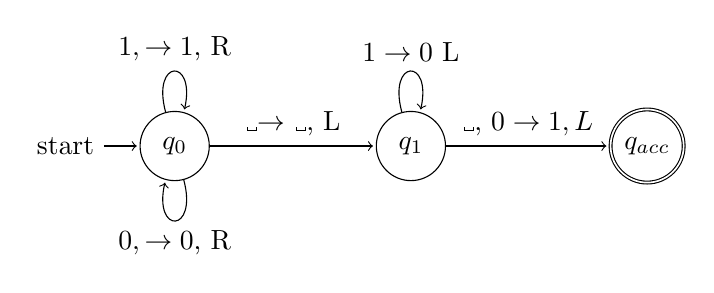
\begin{tikzpicture}[shorten >=1pt,node distance=3cm,on grid,auto]
        \node[state, initial]       (q_0)                                  {$q_0$};
        \node[state]                (q_1)    [right of=q_0]                {$q_1$};
        \node[state, accepting]                (q_acc)    [right of=q_1]                {$q_{acc}$};

        \path[->]   (q_0) edge node {\textvisiblespace $\to$ \textvisiblespace, L} (q_1)
        edge [loop above] node {$1, \to 1$, R} ()
        edge [loop below] node {$0, \to 0$, R} ()
        (q_1) edge node {\textvisiblespace, $0 \to 1, L$} (q_acc)
        edge [loop above] node {$1 \to 0$ L} ()
        ;
    \end{tikzpicture}
\end{question}

\begin{question}
    {1b}
    {Do the same, but if the alphabet is unary. Give the state diagram of a Turing machine which begins with $1^x$ on the tape, and halts with $1^{x+1}$}
    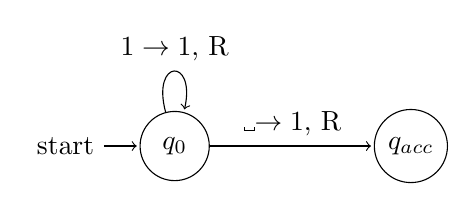
\begin{tikzpicture}[shorten >=1pt,node distance=3cm,on grid,auto]
        \node[state, initial]       (q_0)                                  {$q_0$};
        \node[state]                (q_acc)    [right of=q_0]                {$q_{acc}$};

        \path[->]   (q_0) edge node {\textvisiblespace $\to 1$, R} (q_acc)
        edge [loop above] node {$1 \to 1$, R} ()
        ;
    \end{tikzpicture}
\end{question}

\begin{question}
    {2a}
    {
        For this problem, you will describe a TM $M$ that takes as input a DFA $D$ and an input $x$, and returns whether $D$ accepts $x$.
        For simplicity, assume that the input alphabet for $D$ is $\{0,1\}$. (Note: $D$ is part of the \textit{input}.
        You are not building a different Turing machine for each possible DFA, you are building a single Turing machine that can simulate every DFA.)

        Let $\Sigma_M = \{0,1,\#\}$ be the input alphabet for $M$. An input to $M$ is a ordered pair $(D,x)$.
        Describe an appropriate encoding scheme for the input to $M$.}

    Let $M$ be the multitape Turing machine and $T_i, i=1,2,3,4$ be the four tapes for $M$. They are organised and encoded as follows:
    \begin{itemize}
        \item $T_1$ is simply the input to $D$. Since the input alphabet is just $\set{0,1}$ we can simply copy over this input to $T_1$.
        \item $T_2$ contains the final states of $D$. We will encode any state $q_i$ as $(i)_2$ (i.e., the base 2 representation of $i$) and separate them with ``\#''.
        \item $T_3$ will contain the current state of $D$. Again, we will encode the state $q_i$ as $(i)_2$.
        \item $T_4$ contains the transitions of $D$. Let $a \in \Sigma = \set{0,1}$, we will encode transition $\delta(q_i, a) = q_j$ as $(i)_2\#a\#(j)_2$. We will separate each transition with ``\#\#''
    \end{itemize}
\end{question}

\begin{question}
    {2b}
    {Describe, at a higher level than problem 1, how $M$ runs.  Your description does not need to explain how to check if two strings are equal
        but should otherwise describe the path that the tape head will follow as $M$ runs.}

    The first step is to encode and copy the input, final states, current (start) state, and transitions onto their respective tapes. Then, we rewind
    all the heads to the beginning of the tape. The first step is to find the transition function in $T_4$ that matches the current state and the character in
    the input tape $T_1$. After the right transition function the new state is written onto $T_3$. Then, we move the tape head of $T_1$ one place forward
    to evaluate the new character. We repeat this until the head of $T_1$ hits a blank space. Then, we check whether the current state in $T_3$ is contained
    within $T_2$, and this determines whether we accept or reject the input.
\end{question}

\begin{question}
    {2c}
    { How often does your machine call the ``check if two strings are equal" subroutine?
        Outside of this subroutine, how often does it mark a character (i.e. replace ``$a$" with ``$\dot{a}$")?}

    This Turing Machine never marks characters. String comparison is performed at the end when we compare the state after the input tape reaches a blank
    to every (until found) accepting state in $T_2$. There is also a string comparison performed every time we need to find the transition function
    for a character and a current state.
\end{question}

\begin{question}
    {3}
    {Let a $2L3R$-TM be a Turing Machine that, at each step, either moves the tape head two steps to the left or three steps to the right.
        Show that $2L3R$-TM's are exactly as powerful as Turing Machines by showing, for each type of machine, how to construct an equivalent machine
        of the other type. (Note that this proof has two directions, and you must prove both of them.)}

    ($\Rightarrow$) We will show that a $2L3R$-TM is equivalent to a regular TM. We will do this by showing a $2L3R$-TM can move the same way as a regular
    TM. In fact, to move one position to the left, we can move \emph{twice} to the left (i.e., move head 4 to the left) and move once to the right
    (i.e., move head three steps to the right) to achieve an overall "one to the left" move. To move one position to the right, we can move to the right
    (move the head 3 positions right) and then move left (move head 2 positions left) to achieve an overall "one to the right" movement.

    ($\Leftarrow$) We will show a regular TM is equivalent to a $2L3R$-TM. A regular TM can move two steps to the left by moving one step to the left twice.
    It can move 3 steps to the right by moving one steps to the right three times. Therefore, it is equivalent to a $2L3R$-TM.
\end{question}

\begin{question}
    {4a}
    {An unrestricted grammar is similar to a context-free grammar, except that its rules are of the form $u \rightarrow v$,
        where $u$ and $v$ are \emph{both} strings containing any number of terminals and non-terminals.

        Here is an unrestricted grammar:

        \begin{align*}
            S  & \rightarrow \epsilon \\
            S  & \rightarrow aASCc    \\
            Aa & \rightarrow aA       \\
            cC & \rightarrow Cc       \\
            bC & \rightarrow Cb       \\
            AC & \rightarrow b
        \end{align*}

        What language does this grammar generate?
    }
    The language generated is $\set{a^nb^nc^n: n\geq 0}$.
\end{question}

\begin{question}
    {4b}
    {Let $L$ be a language generated by an unrestricted grammar $G$. Show that $L$ is Turing-recognizable.
        (Do NOT give an example for a specific language. Your answer should be an explanation for how to build an equivalent Turing Machine for any
        unrestricted grammar.)}

    Let $T_1, T_2$ be two tapes to our Turing Machine. $T_1$ contains the input and $T_2$ contains the grammar. Now, we can non-deterministically apply
    the rules from $T_2$ to a non-deterministically chosen position of $T_2$. We do this until $T_2$ matches $T_1$. Now, we know that every multitape
    Turing Machine has a single tape equivalent, hence, we have shown that $L$ is Turing-recognizable.
\end{question}

\begin{question}
    {4c}
    {Show that, for any Turing-recognizable $L$, there is an unrestricted grammar that generates $L$.
        (Hint: We showed in class how to represent the configuration of a Turing machine as a string, i.e. $001q_700$.
        At each step, the configuration of the machine changes. Think about how the configuration string changes,
        and represent this change with a grammar rule.)}

    Let $L$ be the language accepted by a Turing Machine $M = Q, \Sigma, \Gamma, \delta, q_0, q_{acc}, q_{rej}$. We will construct a grammar $G$ that nondeterministically generates two copies of a repressentation of some word in $\Sigma^*$ and simulates the action of $M$ on one copy. If $M$ ends up accepting the copy,
    then $G$ turns the second copy into a terminal string, otherwise this second copy never ends up as a terminal string.

    We let $G = (V, \Sigma, P, A_1)$ be the grammar. Now, we have the productions:
    \begin{enumerate}
        \item $A_1 \to q_0A_2$
        \item $A_2 \to [a, a]A_2, \forall a \in \Sigma | A_3$
        \item $A_3 \to [\epsilon, q_{acc}]A_3 | \epsilon$
        \item $q[a, X] \to [a, Y]p, \forall a \in \Sigma_\epsilon, \forall q \in Q, \forall X, Y \in \Gamma, \delta(q, X) = (p, Y, R)$
        \item $[b, Z]q[a, X] \to p[b, Z][a, Y], \forall X,Y,Z \in \Gamma, \forall a, b \in \Sigma_\epsilon, \forall q \in Q, \delta(q, X) = (p, Y, L)$
        \item $[a, X]q \to qaq, q[a, X] \to qaq, q \to \epsilon, f \forall a \in \Sigma_\epsilon, \forall X \in \Gamma, \forall q \in F$.
    \end{enumerate}

    Now, let $a_i \in \Sigma$ for all $i$ using 1 and 2 we get that $A_1 \to q_0[a_1, a_1][a_2, a_2]\dots[a_n, a_n]A_2$. Now, suppose that
    $M$ accepts the string $a_1a_2\dots a_n$. Then $M$ yses no more than $m$ cells to the right of it's input. Now, we apply rule 3, 4 ($m$ times), and
    5 to get $A_1 \to  q_0[a_1, a_1][a_2, a_2]\dots[a_n, a_n][\epsilon, q_{acc}]^m$. Now, we can simply use rules 6 and 7 until an accepting state is
    generated non-deterministically.

\end{question}
\end{document}